\documentclass[tikz,border=10pt]{standalone}
\usepackage{tikz}
\usetikzlibrary{calc}

\begin{document}
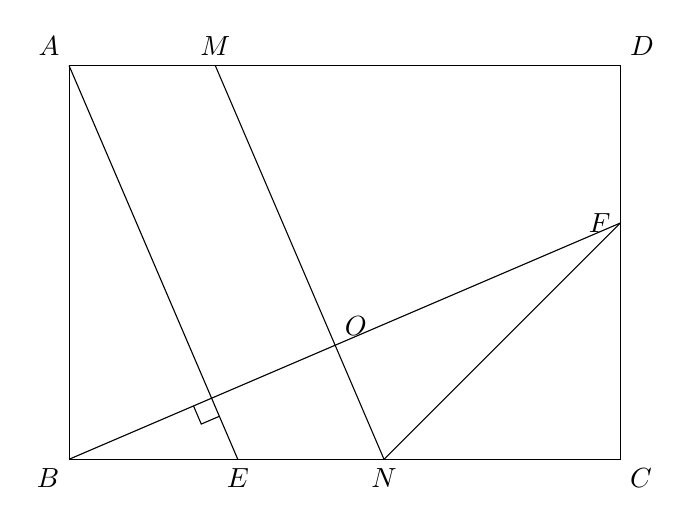
\begin{tikzpicture}
    \coordinate (A) at (0, 5);
    \coordinate (B) at (0, 0);
    \coordinate (C) at (7, 0);
    \coordinate (D) at (7, 5);
    \coordinate (F) at (7, 3);
    \coordinate (E) at (15/7, 0);
    \coordinate (N) at (4, 0);
    \coordinate (M) at (13/7, 5);
    \coordinate (O) at (98/29, 42/29);
    \coordinate (P) at (105/58, 45/58);

    \draw (A) -- (B) -- (C) -- (D) -- cycle;
    \draw (A) -- (E);
    \draw (B) -- (F);
    \draw (M) -- (N);
    \draw (N) -- (F);

    \coordinate (P1) at ($(P)!0.25cm!(B)$);
    \coordinate (P2) at ($(P)!0.25cm!(E)$);
    \draw (P1) -- ($(P1) + (P2) - (P)$) -- (P2);

    \node[above left] at (A) {$A$};
    \node[below left] at (B) {$B$};
    \node[below right] at (C) {$C$};
    \node[above right] at (D) {$D$};
    \node[above] at (M) {$M$};
    \node[below] at (E) {$E$};
    \node[below] at (N) {$N$};
    \node[left] at (F) {$F$};
    \node[above right] at (O) {$O$};
\end{tikzpicture}
\end{document}
